\section{Class diagram}
\subsection{Introduction}
\begin{flushleft}
Cette extension ne change en rien la logique de base que nous avons construite dans la base du projet.
\end{flushleft}

\begin{flushleft}
En effet, les packages : 
\end{flushleft}
\begin{enumerate}
\item Api
\item Database
\item DataObject
\item App
\end{enumerate}
\begin{flushleft}
sont conservés avec la même logique.
\end{flushleft}

\begin{flushleft}
Repassons donc sur les quelques classes et méthodes essentielles rajoutées pour la conception de l'extension.
\end{flushleft}

\subsection{Le package api}
\begin{flushleft}
Dans ce package, vous pouvez trouver l'ajout des méthodes liées aux clients dans \textbf{"ClientApi"} en prenant en compte les nouvelles possibilités liées aux clients invités, aux portefeuilles invités ainsi qu'aux permissions étant accordées.
\end{flushleft}

\begin{flushleft}
Cette classe sera toujours utilisée pour les requêtes liées aux clients lorsqu'ils sont connectés.
\end{flushleft}

\begin{flushleft}
Ils pourront effectuer les opérations qu'ils souhaitent au niveau des :
\end{flushleft}
\begin{enumerate}
\item portefeuilles
\item \textbf{portefeuilles invités}
\end{enumerate}

\begin{flushleft}
et auront également la possibilité de voir tous leurs contrats ainsi que les propositions des fournisseurs.
\end{flushleft}

\newpage
\subsection{Le package dataBase}
\begin{flushleft}
Ce dernier contient toutes les méthodes qui vont communiquer avec la base de données de la base du projet ainsi que celles ajoutées précédemment pour l'extension.
\end{flushleft}

\begin{flushleft}
Comme pour la  base du projet, vous pouvez noter que celles-ci ont exactement le même nom que dans le package API puisqu'elles sont contenues dans la suite du programme.
\end{flushleft}

\begin{flushleft}
Vous pouvez donc observer l'ajout des méthodes dans la classe \textbf{"ClientDB"}.
\end{flushleft}

\subsection{Le package dataObject}
\begin{flushleft}
Ce package reprend les classes représentant un objet, c'est-à-dire pour l'extension :
\end{flushleft}
\begin{enumerate}
\item Les clients
\item Les portefeuilles
\item \textbf{Les portefeuilles invités}
\item Les propositions
\item Les notifications
\end{enumerate}

\begin{flushleft}
Vous pouvez remarquer l'ajout des permissions dans la classe \textbf{"ClientBasic"} et la gestion des clients invités dans \textbf{"WalletFull"}.
\end{flushleft}

\begin{flushleft}
En outre, la création des classes \textbf{"InvitedWalletBasic"} et \textbf{"InvitedWalletFull"} permettent de respecter les choix effectués concernant le fait de séparer les portefeuilles "classiques" des portefeuilles invités.
\end{flushleft}

\newpage
\subsection{Diagramme}
\begin{figure}[h]
\centering
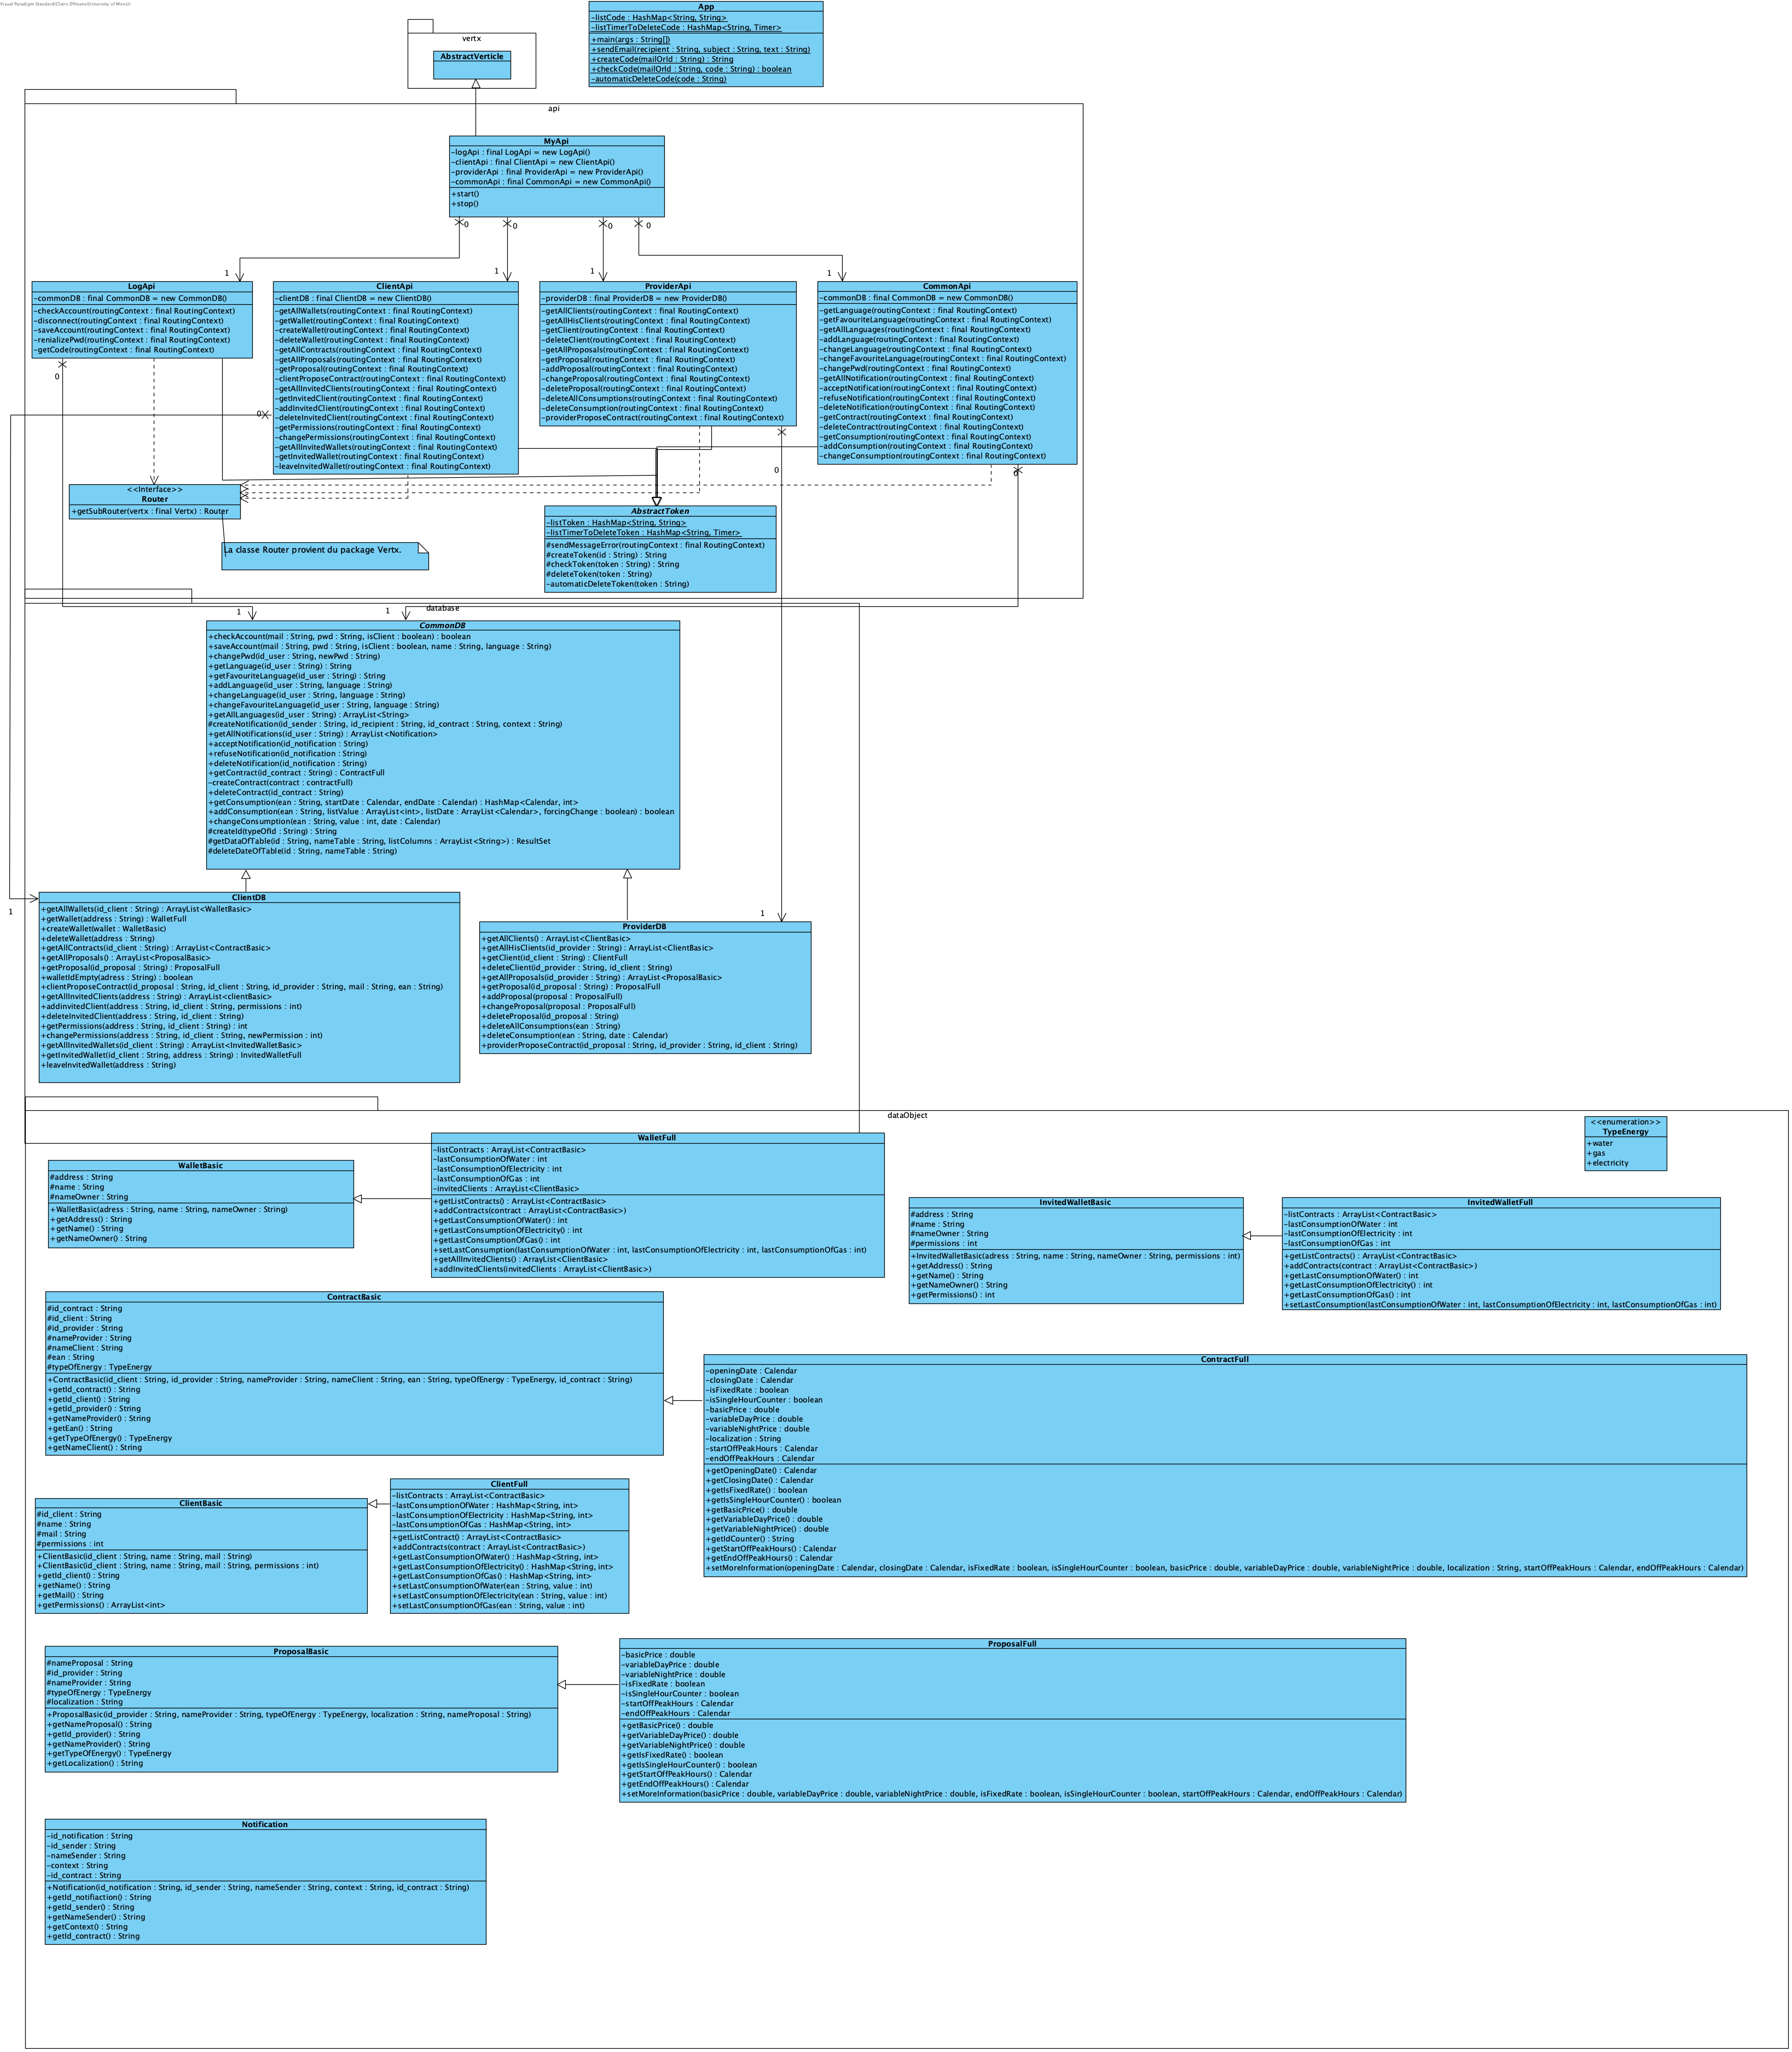
\includegraphics[width = 1\textwidth]{Extension-claire/Class-claire/img/class.png}
\end{figure}
